\documentclass[12pt]{article}
\usepackage[utf8]{inputenc}
\usepackage[english]{babel}
\usepackage{graphicx}
\usepackage{algorithm}
\usepackage{algpseudocode}
\usepackage{hyperref}

\title{Artificial Nose}
\author{Luca Belluardo e Andrea Stevanato}
\date{\today}

\begin{document}

\maketitle
\tableofcontents

\section{Introduction}
In this project a real-time application is developed to recognize smells from an
artificial nose. The sensor used for the application is an air quality gas 
sensor.

The rest of the documentation is structured in the following way: in section
2 the tasks are explained one at a time, in the section 3...

\section{The tasks}
In our application we have 5 periodic tasks (Figure \ref{tdiagram}): graphic
task, sensor task, neural network task (made with Tensorflow), keyboard task
and the store image task.

The main function sets everything up for the tasks, except for the store
image task. The keyboard task is in charge to execute the store image task
when the \texttt{ENTER} key is pressed. If the store image task is already in
execution and the \texttt{ENTER} key is pressed this it's terminated.
Before start the store image task it's possible to write the name of the
directory in which the images will be saved; if no name it's writed the
images will be saved into \textit{image\_neural\_network} directory.

The sensor is readed by an Arduino M0 pro; the sampled data readed by arduino
are sent via the serial port to our application and readed by the sensor
task. All the tasks are terminated by the keyboard task when the user presses
the \texttt{ESC} key.

\begin{figure}[!t]
    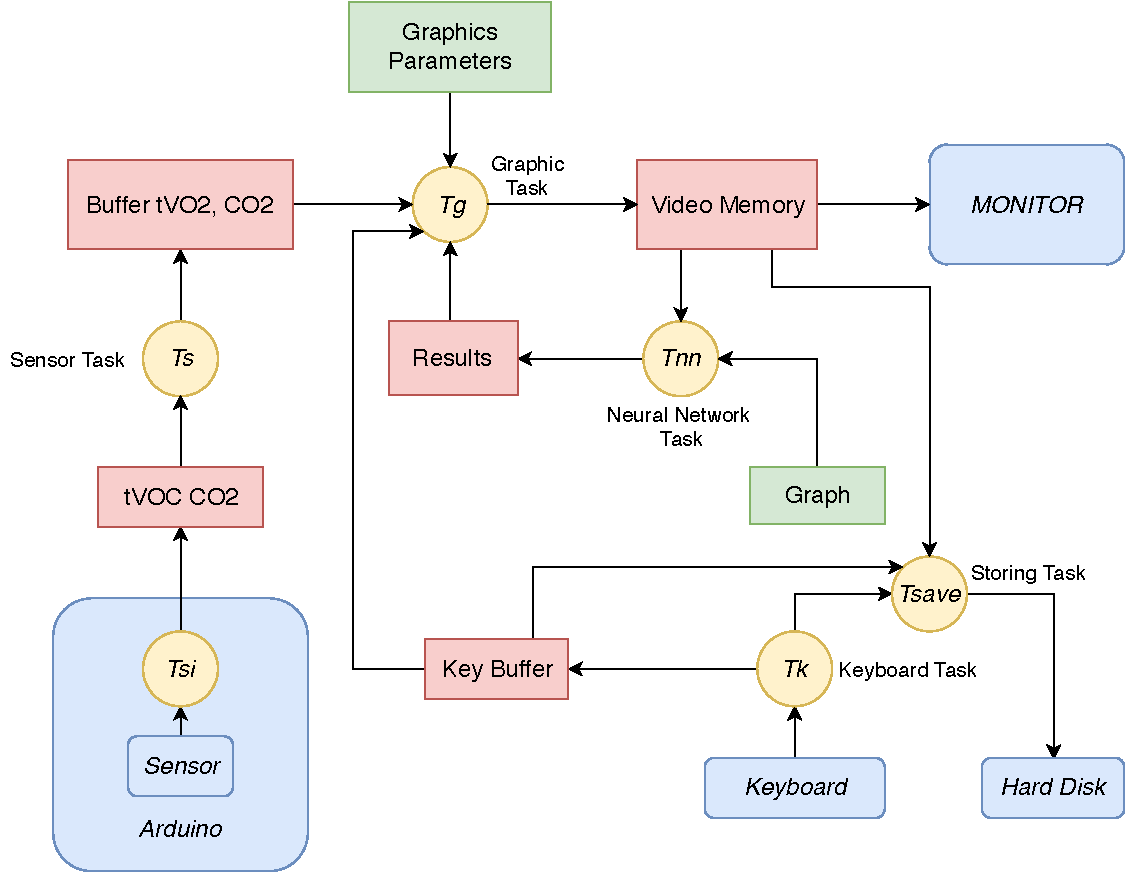
\includegraphics[width=\textwidth]{diagram.pdf}
    \caption{Task diagram}
    \label{tdiagram}
\end{figure}

\subsection{Main function}
In the main function [\ref{main}] all the tasks, except the store image task,
are started and the mutexes initialized. The mutexes are three, one for the
data readed from the sensor, one for the results given by the neural
network and one for the buffer that contains the keyboard input. The main also 
starts allegro and waits for the termination of the
keyboard task. Once the keyboard task terminates the main cancels all other
task and wait for their termination.

\begin{algorithm}[t]
\caption{Main}
\label{main}

\begin{algorithmic}
\State $T\gets$ \textit{tasks to be started}
\State Mutexes and allegro initialization
\For{$t \in T$}
    \State start $t$
\EndFor

\Loop{ \textit{wait for termination of keyboard task}}
\EndLoop

\For{$t \in T$} 
    \State cancel and join $t$
\EndFor

\end{algorithmic}
\end{algorithm}

\subsection{Graphic Task}

The graphic task prints the interface of our application. The
interface is divided into different areas that contains for each one the
graph (Figure \ref{graph}), the image (Figure \ref{image}), the results (Figure \ref{results}), the legend (Figure \ref{legend}), the current values (Figure \ref{values}) and the current
status (\texttt{WRITING} (Figure \ref{writing}) or \texttt{SAVING} (Figure \ref{saving})) followed by, if present, the
keyboard input.

\begin{figure}[!t]
    \centering
    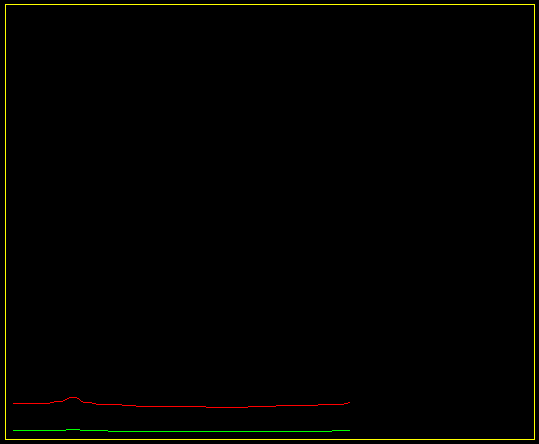
\includegraphics[scale=0.75]{graph.png}
    \caption{Graph}
    \label{graph}
\end{figure}

\begin{figure}[!t]
    \centering
    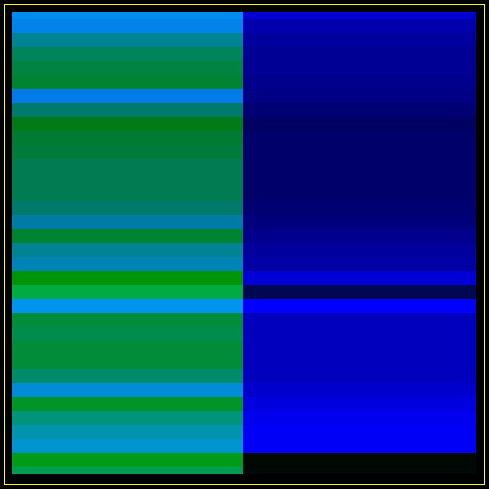
\includegraphics[scale=0.75]{image.png}
    \caption{Image}
    \label{image}
\end{figure}

\begin{figure}[!t]
    \centering
    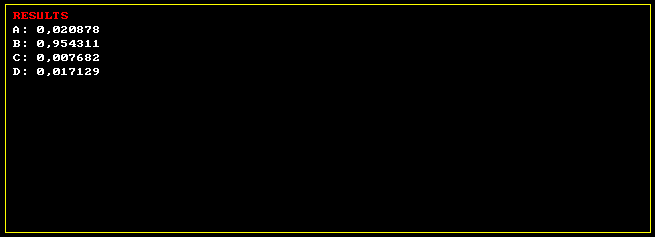
\includegraphics[scale=0.75]{results.png}
    \caption{Result}
    \label{results}
\end{figure}

\begin{figure}[!t]
    \centering
    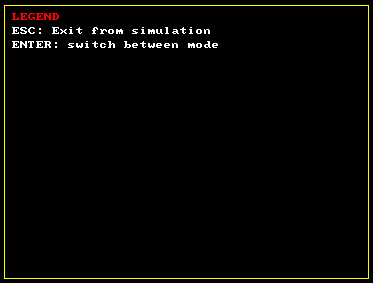
\includegraphics[scale=0.75]{legend.png}
    \caption{Legend}
    \label{legend}
\end{figure}

\begin{figure}[!t]
    \centering
    
\includegraphics[scale=0.75]{values.png}
    \caption{Current values}
    \label{values}
\end{figure}

\begin{figure}[!t]
    \centering
    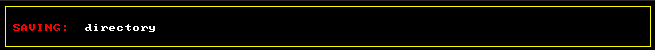
\includegraphics[scale=0.75]{saving.png}
    \caption{Saving mode}
    \label{saving}
\end{figure}

\begin{figure}[!t]
    \centering
    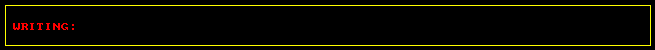
\includegraphics[scale=0.75]{writing.png}
    \caption{Writing mode}
    \label{writing}
\end{figure}

\begin{algorithm}[t]
\caption{Graphic task}
\label{graphic}
\begin{algorithmic}
\State $p\gets$ \textit{task period}
\State set activation task
\State draw interface background

\Loop
\State draw graph
\State draw image
\State draw results given by neural network
\State draw current values readed from sensor
\State draw keyboard input
\State wait for next activation
\EndLoop

\end{algorithmic}
\end{algorithm}

\subsection{Sensor task}
The sensor task [\ref{sensortask}] reads the values from the arduino which it
sends on serial port the values given by the sensor. The readed values are
stored into an array and used by the graphic task to draw the image and the
graph; the current readed values are also standalone printed by the graphic
task.

\begin{algorithm}[t]
\caption{Sensor task}
\label{sensortask}

\begin{algorithmic}
\State $p\gets$ \textit{task period}
\State initialization $data\_q$
\State initialization serial port
\State set activation task

\Loop
\State $data\_q\gets data\_q$ + values readed from sensor
\State wait for next activation
\EndLoop

\end{algorithmic}
\end{algorithm}

\subsection{Neural network task}
The neural network task [\ref{nntask}] recognizes the smells using the
current image created with the value sampled from sensor.

\begin{algorithm}[t]
\caption{Neural network task}
\label{nntask}

\begin{algorithmic}
\State $p\gets$ \textit{task period}
\State Tensorflow initialization
\State set activation task

\Loop
\State $image\gets$ current image
\State $results\gets$ use neural network with given $image$
\State wait for next activation
\EndLoop

\end{algorithmic}
\end{algorithm}

\subsection{Keyboard task}
The keyboard task [\ref{ktask}] takes input from keyboard and
put it into \textit{keyboard buffer}. The keyboard buffer is printed by the
graphic task in its area of interface. The string contained into keyboard
buffer is the directory, under \textit{image\_neural\_network}, where the
images are saved by the store image task. The keyboard task shall be in two
different mode: \texttt{WRITING} or \texttt{SAVING}. The task is started in
\texttt{WRITING} mode. During this mode it's possible to write the name of
the directory in which the images are saved. The name can contain letters,
numbers, minus, underscore and point; it's also possible to delete the written
characters pressing the \texttt{BACKSPACE} key. Pressing the
\texttt{ENTER} key, the current mode is switched from the \texttt{WRITING} to
the \texttt{SAVING} mode or vice versa. When the \texttt{ESC} key is pressed the
task terminate causing the closing of our application.

\begin{algorithm}[t]
\caption{Keyboard task}
\label{ktask}

\begin{algorithmic}
\State $p\gets$ \textit{task period}
\State $cur\_mode\gets$ \texttt{WRITING}
\State create \textit{key\_buffer}
\State keyboard initialization
\State set activation task

\Repeat
\State $key\_pressed\gets$ key code from keyboard
\If {$key\_pressed$ == \texttt{ENTER}}
    \If {$cur\_mode$ == \texttt{WRITING}}
    \State $cur\_mode\gets$ \texttt{SAVING}
    \State start store image task
    \Else
    \State $cur\_mode\gets$ \texttt{WRITING}
    \State stop store image task and clean key\_buffer
    \EndIf
\ElsIf {$cur\_mode$ == \texttt{WRITING}}
    \If {$key\_pressed$ equal to letter, number, minus or point \textbf{and} \textit{key\_buffer} not full}
        \State \textit{key\_buffer} $\gets$ \textit{key\_buffer} + $key\_pressed$ 
    \ElsIf {\textit{key\_buffer} == \texttt{BACKSPACE} \textbf{and} \textit{key\_buffer} not empty}
        \State remove last element from \textit{key\_buffer}
    \EndIf
\EndIf

\Until {$key\_pressed$ != \texttt{ESC}}

\end{algorithmic}
\end{algorithm}

\subsection{Store image task}
The store image task [\ref{sitask}] is activated/terminated by keyboard task
when the \texttt{ENTER} key is pressed. Once the task is activated the image
are saved every $300$ milliseconds. The images saved by this task are used to
train the neural network for the recognizing of smells.

\begin{algorithm}[t]
\caption{Store image task}
\label{sitask}

\begin{algorithmic}
\State $p\gets$ \textit{task period}
\State $dir\gets$ \textit{path to directory where images are saved}
\State set activation task

\Loop
\State save image to $dir$
\State wait for next activation
\EndLoop

\end{algorithmic}
\end{algorithm}

\subsection{Scheduling}
\subsection{Count deadline}

\section{Creation image}
The image is created from the values readed from the sensor. The allegro color 
mode is set to 16 bits. In the 16 bits mode 5 bits are for the red and blue 
values e 6 bits for the green value. 

The sensor samples two data, the CO2 and the tVOC. Each value is a 16-bit number
and so we represent the values readed as colors in 16-bit. The image is splitted
in two parts, left and right. In the left side we draw the CO2 and in the right 
the tVOC.

Whenever we read a new pair of values from the sensor, we move the previous 
image one line below, removing the line at the bottom of the image, and we add 
the new line on the top of the image.

\section{Focus on neural network}
Regarding the neural network we used Tensorflow, an open-source software 
library for dataflow programming across a range of tasks. 

For training the neural network we used a python code \cite{retrain} provided by
Tensorflow. In this file a lot of configurations are possible. In our 
application we use the default configurations and choose only the number of 
training steps.

\section{Neural network training}

\section{The results}

\section{Conclusions}

\begin{thebibliography}{9}
\bibitem{retrain}How to Retrain an Image Classifier for New Categories 
\texttt{\hyperlink{How to Retrain an Image Classifier for New 
Categories}{https://www.tensorflow.org/hub/tutorials/image\_retraining}}

\end{thebibliography}

\end{document}
